\documentclass[tikz,border=8pt]{standalone}
\usepackage[T1]{fontenc}
\usepackage{helvet}
\renewcommand{\familydefault}{\sfdefault}
\usetikzlibrary{arrows.meta}

\definecolor{queryfill}{HTML}{DFF7F3}
\definecolor{queryborder}{HTML}{1BA99C}
\definecolor{corpusfill}{HTML}{FFF4D6}
\definecolor{corpusborder}{HTML}{D9A441}
\definecolor{embedfill}{HTML}{E9EDFF}
\definecolor{embedborder}{HTML}{6979C9}
\definecolor{storefill}{HTML}{E8F2FF}
\definecolor{storeborder}{HTML}{4E8CD8}
\definecolor{rerankfill}{HTML}{FFE9C8}
\definecolor{rerankborder}{HTML}{D88922}
\definecolor{outfill}{HTML}{E7F6E7}
\definecolor{outborder}{HTML}{4FA64F}
\definecolor{softgray}{HTML}{F4F7FB}
\definecolor{darkline}{HTML}{333333}

\tikzset{
  card/.style={rectangle, rounded corners=5pt, align=center, draw=darkline, line width=0.8pt, minimum height=0.82cm, font=\small},
  query/.style={card, fill=queryfill, draw=queryborder, minimum width=2.05cm},
  corpus/.style={card, fill=corpusfill, draw=corpusborder, minimum width=2.35cm},
  embed/.style={card, fill=embedfill, draw=embedborder, minimum width=2.7cm, font=\small\bfseries},
  store/.style={card, fill=storefill, draw=storeborder, minimum width=2.65cm, font=\small\bfseries},
  rerank/.style={card, fill=rerankfill, draw=rerankborder, minimum width=2.8cm, font=\small\bfseries},
  artifact/.style={card, fill=white, minimum width=2.75cm},
  output/.style={card, fill=outfill, draw=outborder, minimum width=2.75cm},
  softbox/.style={rectangle, rounded corners=8pt, draw=darkline, fill=softgray, line width=0.7pt},
  doc/.style={rectangle, rounded corners=4pt, fill=corpusfill, draw=corpusborder, line width=0.7pt, minimum width=0.42cm, minimum height=0.58cm},
  vec/.style={rectangle, rounded corners=2pt, fill=storefill, draw=storeborder, line width=0.65pt, minimum width=0.16cm, minimum height=0.72cm},
  node/.style={circle, fill=storefill, draw=storeborder, line width=0.7pt, minimum size=0.29cm},
  finalnode/.style={circle, fill=outfill, draw=outborder, line width=0.7pt, minimum size=0.29cm},
  phase/.style={font=\small\bfseries, align=center},
  lane/.style={font=\scriptsize\bfseries, align=center},
  flow/.style={-{Latex[length=2.2mm]}, line width=0.85pt, draw=darkline},
  faint/.style={dashed, darkline, opacity=0.32}
}

\begin{document}
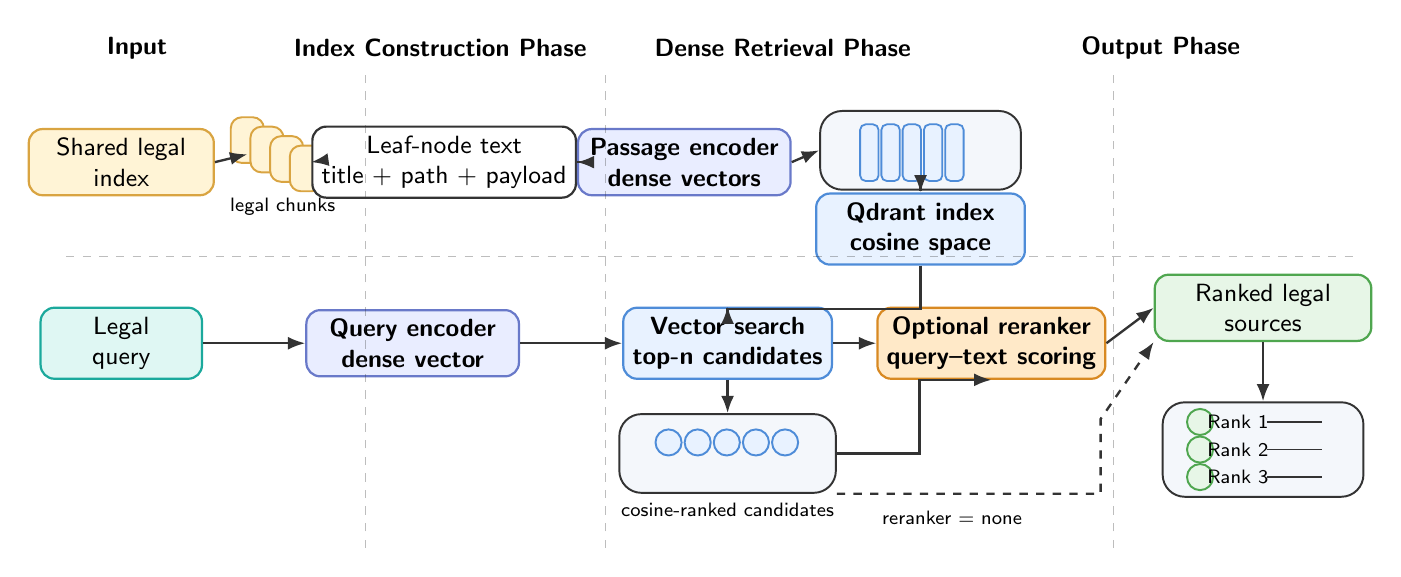
\begin{tikzpicture}

\node[phase] at (1.05,6.35) {Input};
\node[phase] at (4.9,6.35) {Index Construction Phase};
\node[phase] at (9.25,6.35) {Dense Retrieval Phase};
\node[phase] at (14.05,6.35) {Output Phase};

% Offline indexing lane.
\node[corpus] (corpus) at (0.85,4.9) {Shared legal\\index};
\foreach \x/\y in {2.45/5.18,2.7/5.06,2.95/4.94,3.2/4.82} {
  \node[doc] at (\x,\y) {};
}
\node[font=\scriptsize] at (2.9,4.34) {legal chunks};

\node[artifact] (chunks) at (4.95,4.9) {Leaf-node text\\title + path + payload};
\node[embed] (passageembed) at (8.0,4.9) {Passage encoder\\dense vectors};

\node[softbox, minimum width=2.55cm, minimum height=1.0cm] (qdrantbox) at (11.0,5.05) {};
\foreach \x in {10.35,10.62,10.89,11.16,11.43} {
  \node[vec] at (\x,5.02) {};
}
\node[store] (qdrant) at (11.0,4.05) {Qdrant index\\cosine space};

% Online retrieval lane.
\node[query] (query) at (0.85,2.6) {Legal\\query};
\node[embed] (queryembed) at (4.55,2.6) {Query encoder\\dense vector};
\node[store] (search) at (8.55,2.6) {Vector search\\top-n candidates};

\node[softbox, minimum width=2.75cm, minimum height=1.0cm] (candidatebox) at (8.55,1.2) {};
\foreach \x in {7.8,8.17,8.54,8.91,9.28} {
  \node[node] at (\x,1.34) {};
}
\node[font=\scriptsize] at (8.55,0.48) {cosine-ranked candidates};

\node[rerank] (reranker) at (11.9,2.6) {Optional reranker\\query--text scoring};
\node[output] (sources) at (15.35,3.05) {Ranked legal\\sources};
\node[softbox, minimum width=2.55cm, minimum height=1.2cm] (rankbox) at (15.35,1.25) {};
\foreach \y/\lab in {1.6/1,1.25/2,0.9/3} {
  \node[finalnode] at (14.55,\y) {};
  \node[font=\scriptsize] at (15.03,\y) {Rank \lab};
  \draw[darkline, line width=0.5pt] (15.4,\y) -- (16.1,\y);
}

% Main flows.
\draw[flow] (corpus.east) -- (2.45,5.0);
\draw[flow] (3.4,4.92) -- (chunks.west);
\draw[flow] (chunks.east) -- (passageembed.west);
\draw[flow] (passageembed.east) -- (qdrantbox.west);
\draw[flow] (qdrantbox) -- (qdrant);

\draw[flow] (query.east) -- (queryembed.west);
\draw[flow] (queryembed.east) -- (search.west);
\draw[flow] (qdrant.south) -- ++(0,-0.55) -| (search.north);
\draw[flow] (search) -- (candidatebox);
\draw[flow] (search.east) -- (reranker.west);
\draw[flow] (candidatebox.east) -- ++(1.05,0) |- (reranker.south);
\draw[flow] (reranker.east) -- (sources.west);
\draw[flow] (sources) -- (rankbox);

% Pass-through path for configurations without reranking.
\draw[flow, dashed] (candidatebox.south east) -- ++(3.35,0) -- ++(0,0.95) -- (sources.south west);
\node[font=\scriptsize, align=center] at (11.4,0.38) {reranker = none};

\draw[faint] (3.95,0.0) -- (3.95,6.05);
\draw[faint] (7.0,0.0) -- (7.0,6.05);
\draw[faint] (13.45,0.0) -- (13.45,6.05);
\draw[faint] (0.15,3.7) -- (16.55,3.7);

\end{tikzpicture}
\end{document}
